\documentclass[12pt, a4paper]{article}

\usepackage{fancyhdr}
\usepackage[left=4cm, right=4cm, top=4cm, bottom=4cm]{geometry}
\usepackage[utf8]{inputenc}
\usepackage{amsmath, amssymb, amsthm, amsfonts}
\usepackage{graphicx}
\usepackage{float}
\usepackage{hyperref}
\usepackage{listings}
\usepackage{color}
\usepackage{subcaption}
\usepackage{enumitem}
\usepackage{mathtools}
\usepackage{bbm}
\usepackage{cite}
\DeclareMathOperator*{\argmin}{arg\,min}
\DeclareMathOperator*{\argmax}{arg\,max}

\begin{document}

\begin{center}
    \Large\textbf{Model Card: DenseNet121}\\[0.3cm]
\end{center}

\section{Model Overview}
\textbf{Architecture:} DenseNet121 builds dense connections between layers within each block, allowing each layer to receive input from all preceding layers. This design encourages feature reuse and improves parameter efficiency, which contributes to its competitive performance.\\[0.3cm]
\textbf{Training Data:} The model is trained on the ASL Alphabet dataset containing 87,000 images resized to 200x200 pixels, spanning 29 classes (26 letters plus 3 additional classes to aid live classification).\\[0.3cm]
\textbf{Hyperparameters:}
\begin{itemize}
    \item Optimizer: Adam
    \item Loss Function: Categorical Cross-Entropy
    \item Learning Rate: 0.01
    \item Batch Size: 64
    \item Epochs: 20 (best validation accuracy is chosen)
\end{itemize}
\begin{figure}[H]
    \centering
    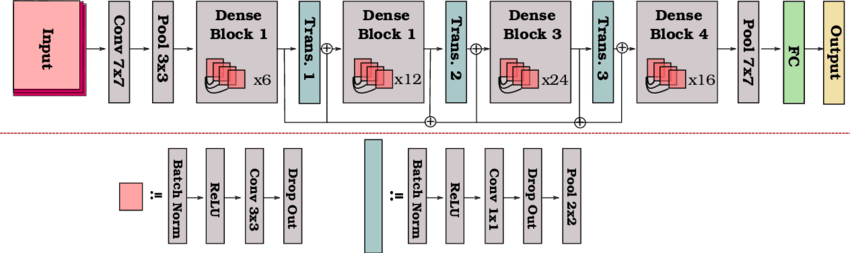
\includegraphics[width=\textwidth]{../../plots/densenet_architecture.png}
    \caption{DenseNet121 Architecture  \cite{denseSparseStateEstimation}}
    \label{fig:resnet18_architecture}
\end{figure}
\begin{figure}[H]
    \centering
    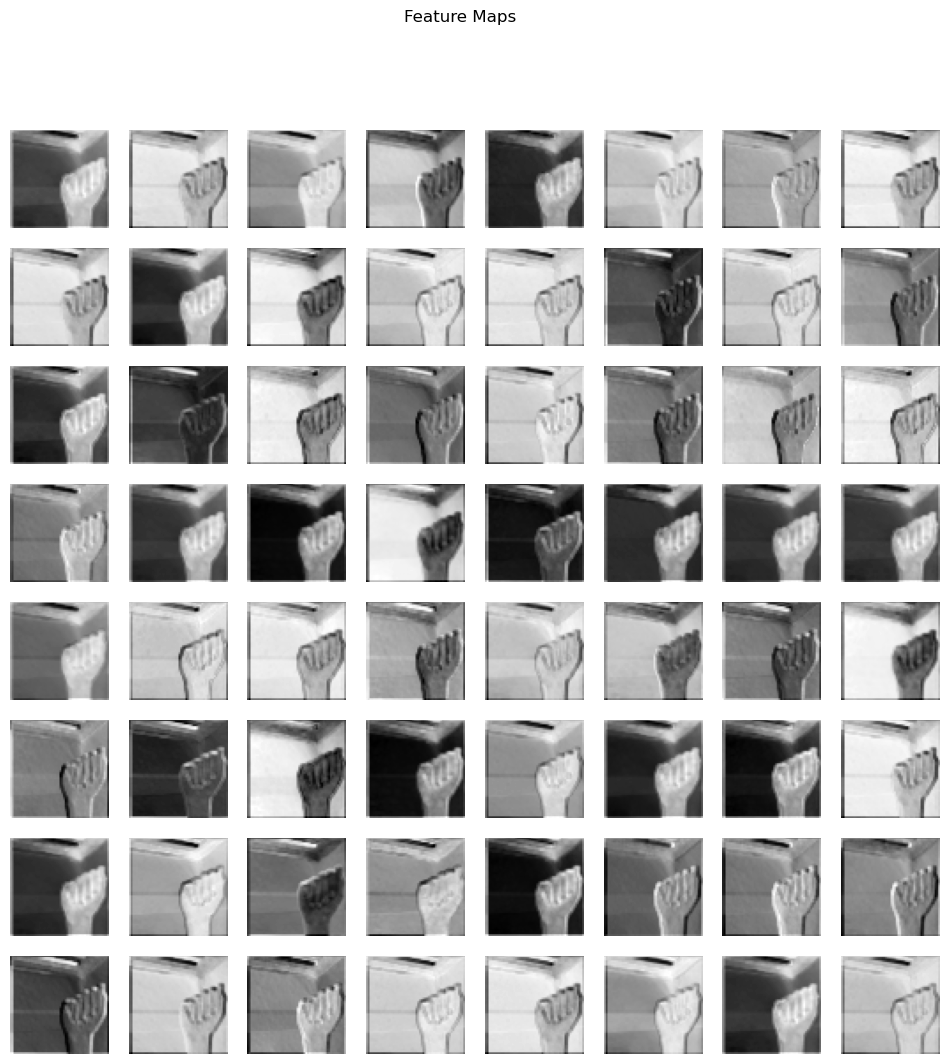
\includegraphics[width=\textwidth]{../../plots/DenseNet121_Visualize.png}
    \caption{DenseNet121 Feature Maps}
    \label{fig:densenet121_visualize}
\end{figure}
\begin{figure}[H]
    \centering
    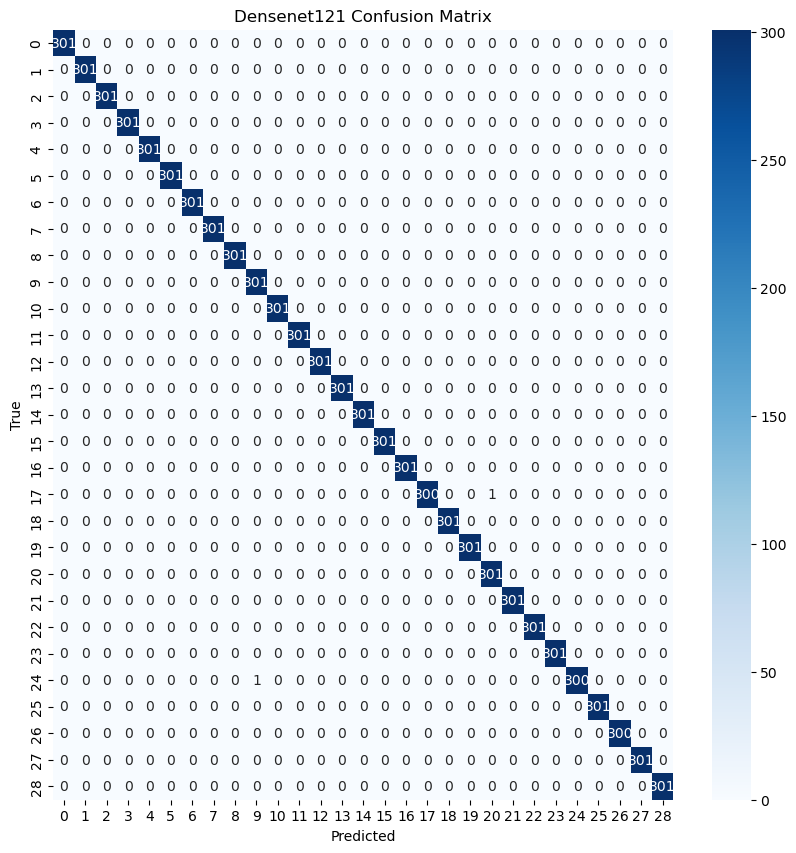
\includegraphics[width=0.8\textwidth]{../../plots/DenseNet121_ConfusionMatrix.png}
    \caption{Confusion Matrix for DenseNet121}
    \label{fig:densenet121_confusion_matrix}
\end{figure}
\section{Intended Use}
DenseNet121 is applied to image classification for American Sign Language (ASL) alphabet letters using a pre-trained model and fine-tuning through transfer learning. The model is intended for:
\begin{itemize}
    \item Classifying ASL alphabet hand signs from static images
    \item Real-time sign language interpretation using live video inputs
\end{itemize}

\section{Performance}
On an independent test dataset, DenseNet121 achieved:
\begin{itemize}
    \item \textbf{Test Accuracy:} 99.98\%
    \item \textbf{Precision:} 1.0
    \item \textbf{Recall:} 1.0
\end{itemize}
DenseNet121’s high performance underscores its capability for near-perfect classification, making it well-suited for both offline and live video recognition tasks.

\section{Limitations}
While achieving high accuracy, DenseNet121 has the following limitations:
\begin{itemize}
    \item Sensitivity to variations in image quality and lighting conditions during live classification
    \item Dependence on precise hand positioning for accurate real-time classification
    \item Practical challenges when deploying on resource-constrained devices
\end{itemize}

\section{Ethical Considerations}
\begin{itemize}
    \item Ensure the ASL dataset is diverse and representative to avoid biased outcomes
    \item Implement privacy protections when deploying real-time video classification systems
\end{itemize}

\bibliographystyle{IEEEtran}
\bibliography{references}
\end{document}
